\chapter*{Conclusion}
\addcontentsline{toc}{chapter}{Conclusion} \markboth{CONCLUSION}{}
\label{sec:final-conclusion}

% Introduce the conclusion
Electrostatic discharges are a major source of stress for electronic devices.
They can cause hardware failures, damaging permanently devices.
This class of issues has been studied for ten years, and is still the core of \gls{esd} research.
Recently, a new class of failures started to be considered.
Electrostatic discharges can cause temporary disturbances on devices.
Most recent integrated technologies enable large performances and massive integration, but also makes more challenging the protection of integrated circuits against external disturbances.
In the same time, electronic modules have increasingly large responsibilities in regard of our safety.
New trends for the autonomous car require electronic devices to take vital decisions for controlling the vehicle.
Guarantying safety of operation against electrostatic discharge is critical.

% Overview of the document
This document detailed three years of research about functional robustness of integrated circuits against electrical transient disturbances.
This field of research is relatively recent, and brings new challenges for \gls{esd} teams in integrated circuit design companies.
During those three years, it became clearer that solving efficiently soft-failure issues requires dedicated tools.
Those tools should enable broader interactions between circuit design team and \gls{esd} team.
They should help detecting and localizing functional weaknesses inside the integrated circuit.
They should also enable better collaboration between integrated circuit companies and equipment manufacturers to design robust boards and applications.
Many tools were studied and proposed throughout this research work.
All the different topics are synthesized in Fig. \ref{fig:phd-map-conclu} that was also presented in the introduction.

\begin{figure}[!h]
  \centering
  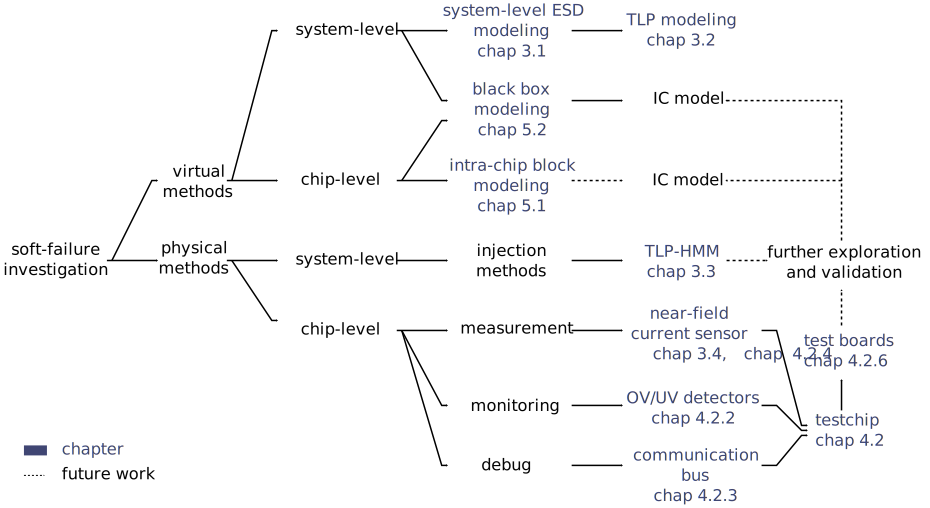
\includegraphics[width=\textwidth]{src/1/figures/structure_of_phd.pdf}
  \caption{Explored research paths for soft-failure investigation and prediction}
  \label{fig:phd-map-conclu}
\end{figure}

% Chap 1
Chapter \ref{chap:1} is a review of the state of the art in ESD testing and soft-failure analysis.
It starts by describing common and recurrent test methods in the ESD field, and identifies relevant and realistic stress sources employed in laboratory environment.
A review of the literature on soft-failure analysis and prediction method is conducted afterward.
It showed that to this day there are rather few research on the topic of ESD-induced soft-failures at silicon level.
Many general-purpose observation techniques exist such as EMMI and near-field scan.
Among the simulation tools, it is common to find \gls{spice} simulation of course, and more advanced techniques such as 3D full-wave electromagnetic simulations or \gls{tcad} simulations.
These tools are highly interesting at the system and board level, to evaluate what fraction of an incoming discharge actually reach an integrated circuit.
It is important to notice that no solution exists so far to investigate at chip level how functions are disturbed by electrostatic discharges.
This point is a key part of the research presented in this document.

% Chap 2
In chapter \ref{chap:2}, a modeling method of electronic systems for ESD is detailed.
It relies and brings a few improvement over existing research conducted in the past on this topic.
A modular approach is employed, where each component is modeled individually to form a library, then assembled together in a hierarchical fashion.
Mostly physically based and most parameters can be extracted with simple tools, or by estimation where it is sometimes enough.
A concrete case study is presented with the modeling of a complex TLP generator.
It is perfect to illustrate a few key points for the modeling methods, and to demonstrate its accuracy against a lot of reference measurements.

% TLP-HMM
The development of this model and the insights gained in the process led to the development of a new pulse generator.
It reproduces the HMM waveform, one of the most widely used test pulse in the ESD field, but in a shielded and controlled environment.
The benefits are increased reproducibility of testing results and a flexibility for shaping the pulse waveform.
The prototype helped identified early issues and improvement to make.

% Correlation method
When comparing this generator to actual ESD guns and standard TLP, a new correlation method has been discovered.
It was validated successfully on 10 different ESD protections.
Correlation methods between ESD generators are extremely valuable because they can ultimately reduce testing time.
By testing a part with a single generator it is possible to predict the failure levels found with the others.
Before being able to do so, the correlation method should be tested on a much larger set of ESD protection.
Failure analysis on the destroyed parts should be conducted to verify if the failure mechanism remains identical between the different generator.

% Near-field current processing
In the last part of chapter \ref{chap:2}, a detailed post-processing method for on-chip near-field sensor has been presented.
It details the operation of the post-processing pipeline developed for this kind of sensor.
The processing script is released \cite{nfs-repository} under an open-source license to promote collaboration and future improvements on the topic.
Two different methods are evaluated and compared in order to reconstitute a current waveform from the voltage measured across the on-chip sensor.

% Chap 3
Chapter \ref{chap:3} presents a real case study where a complex analog function goes into restart because of an ESD.
The function is a primary regulator supply from a large automotive product.
It is put in a lowered \gls{bom} configuration where the external filtering is reduced to diminish the total application cost.
The ESD robustness of this configuration is studied, and a new failure is observed and explained.
After this analysis, it was decided to build a custom chip integrating this particular function, alongside with custom monitoring structures.
There were multiple objectives for making this test vehicle.
The first goal was to acquire waveforms inside the chip, using on-chip measurement structures and sensors, to validate that standard circuit simulations can be employed during an ESD event.
The second goal was to determine when and how analog function were disturbed by transient events, by using custom error detection cells.
This data was meant to validate the modeling methods presented later in the document (in chapter \ref{sec:methods-operating-esd-analysis}).
Creating an entire chip with custom cell design and block reuse, alongside with two application boards was extremely challenging, especially with limited resources and the constraints inherent to the test vehicle process.
Despite extensive testing and validation, issues were met with the communication system responsible for outputting measurement data.
However, the two regulation functions and the on-chip sensors worked properly.
The extensive feedback and knowledge gained from the development of this custom chip is a ground work for new versions of this test vehicle and soft-failure research at silicon-level in general.
It should help define testchip architectures in the future, and with the appropriate fixes the communication system will constitute a reusable and convenient framework for interacting with on-chip monitoring systems.

% Chapter 4
Chapter \ref{sec:methods-operating-esd-analysis} is mainly focused on the development of tools for simulation environment.
The value of simulation tools is well known, because it enables to detect issues very early in the development cycle, which is extremely valuable for avoiding late issues and cutting the cost of fixing them late.
The main challenge for ESD at silicon-level is the complexity of the circuits and simulations.
Convergence issues are very common and sometimes extremely difficult to avoid.
Circuit complexity makes finding issues manually extremely hard.
Most of the time, it is required to manufacture a first silicon to test the parts against ESD and identify soft-failures.
To avoid very costly re-design and late fixes, new methods are required.
In this research, two methods were developed and are described in detail.

% First modelling method
The first method targets analysis and soft-failure prediction of analog function inside the chip, to detect weak spots during early design phase.
It is constituted of two steps, a preliminary characterization and block modeling followed by a chaining process to connect multiple models together and predict their combined robustness.
The characterization is performed by injecting variable amplitude and variable width rectangular pulses.
This characterization results in two different tables, that constitute the block model.
Those tables or model can later be used to determine the response of the block on an output when an input is exposed to a stimulus.
With multiple blocks, stimuli can be propagated from block to block, allowing to predict the shape of the waveform on the final output, just by knowing the waveform on the initial input.
This approach was tested successfully on the test vehicle detailed previously.
It has enabled to predict a failure on the regulator, for different input stresses inject on the battery input.
In summary, this method was validated on a complex analog function coming directly from a real automotive product, and has made possible to predict the ESD robustness of this function using a purely behavioral model.

% Second modelling approach
The second modeling method is more focused on facilitating cooperation between IC manufacturers and equipment manufacturers.
It integrates well inside the SEED methodology, where interaction between these two actors helps design robust products against ESD with optimal cost and development time.
The objective is to characterize and model the relationship between an input pin and an output pin, and to check if a board simulation can be conducted with this black-box IC model.
It was shown that a TLP characterization constitutes a good base for a pin model, in particular for modeling input pins.
For output pins that are supposed to drive a potential in DC conditions, it was demonstrated that this method does not work and requires modifications.
The I(V) curve extracted with the TLP combined with a DC model fails to drive correctly the output voltage and current.
It is an interesting result that calls for more research on this topic.

% Final Conclusion
This research work is one of earliest studies on the topic of ESD-induced functional failures of integrated functions.
It is probably the first to propose analysis and modeling methods at chip level capable of predicting the propagation of a disturbance through multiple analog block functions.
The proposed simulation methods have shown great potential, and open up for many subsequent work and research.
In particular, future work on the model-chain method could involve:

\begin{enumerate}
  \item Simplification of waveforms into rectangular shapes: Waveforms are approximated by a single rectangular pulse.
  It was shown that some waveforms could be approximated better with multiple rectangular shapes.
  It is necessary to study if those multiple shapes could be applied on the model chain input and recombined at the end to deduce the impact of a complex input disturbance.
  Those potential improvements could improve further the accuracy of the model chain.
  \item More robust characterization method: The influence of all elements of the characterization setup should be studied, and eventually taken into account in the model. The goal is to ensure that it is truly the block function that is being characterized, and that the characterization circuit does not interfere or impact the results. Ultimately, the model will be more portable and reusable.
  \item Support of interactions between multiple pins: so far, the characterization is performed with one input and one output.
  It enables to apply a stimulus on an input pin and deduce the signal on an output pin.
  The response on multiple output pins should be also be studied and modeled when multiple input pins are disturbed.
  It could enable to be complete models of analog functions that could reproduce the entire propagation of a fault inside the chip.
\end{enumerate}

This concludes this study on the analysis and prediction of losses of functionality of analog integrated functions induced by electrostatic discharges.
It is a first work that has explored many different approaches and has opened up new leads for future research work.
